\subsection{HTTP Interface}
The client side HTTP interface will use the built in Fetch JavaScript functionality to send and receive resources from and to the server.

\begin{figure}[h!]
	\centering
 	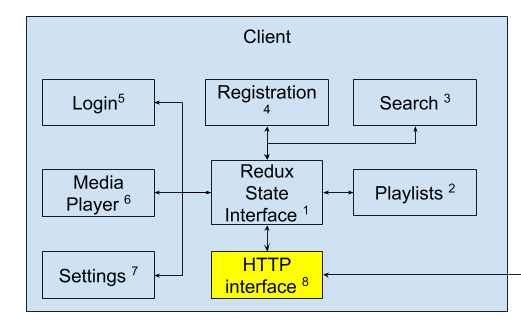
\includegraphics[width=0.60\textwidth]{images/client/client_http_interface.png}
 	\caption{Client-side HTTP interface subsystem}
\end{figure}

\subsubsection{Assumptions}
We will assume we are using the latest version of NodeJS and React on the client side that contains the dependencies.  

\subsubsection{Responsibilities}
This interface will be responsible for sending and receiving requests from the server, as well as interacting with Redux to keep the state of the application in sync. This interface will be involved in logging in, registering, streaming songs from the third party services, and sending updates/creation of playlists to the server.

\subsubsection{Subsystem Interfaces}
\begin {table}[H]
\caption {Client-side HTTP Interface interfaces} 
\begin{center}
    \begin{tabular}{ | p{1cm} | p{6cm} | p{3cm} | p{3cm} |}
    \hline
    ID & Description & Inputs & Outputs \\ \hline
    \#01 & Description of the interface/bus & \pbox{3cm}{Input 1 \\ Input 2} & \pbox{3cm}{Output 1}  \\ \hline
    \#02 & Description of the interface/bus & \pbox{3cm}{N/A} & \pbox{3cm}{Output 1}  \\ \hline
    \end{tabular}
\end{center}
\end{table}

\newpage